\documentclass[11pt,a4paper]{article}
\usepackage[left=24mm,right=24mm,top=20mm,bottom=20mm,headheight=14pt]{geometry}
\usepackage[T1]{fontenc}
\usepackage{lmodern}
\usepackage{microtype}
\usepackage{amsmath,amssymb}
\usepackage{graphicx}
\graphicspath{{figures/}}
\usepackage{booktabs}
\usepackage{fancyhdr}
\usepackage{xcolor}
\usepackage[colorlinks=true,linkcolor=blue!50!black,citecolor=blue!50!black,urlcolor=blue!50!black]{hyperref}
\usepackage{caption}
\captionsetup{font=small,labelfont=bf}
\setlength{\parindent}{1.5em}
\setlength{\parskip}{0pt}
\setlength{\textfloatsep}{12pt plus 2pt minus 2pt}
\setlength{\intextsep}{12pt plus 2pt minus 2pt}
\pagestyle{fancy}
\fancyhf{}
\fancyhead[L]{\small Hawking evaporation and Bondi accretion}
\fancyhead[R]{\small E. Anaraly uulu}
\fancyfoot[C]{\thepage}
\renewcommand{\headrulewidth}{0.3pt}
\newcommand{\Mcrit}{M_{\mathrm{crit}}}
\newcommand{\tstar}{t_*}
\newcommand{\taubb}{\tau_{\mathrm{bb}}}
\newcommand{\Pbb}{P_{\mathrm{bb}}}
\newcommand{\Msun}{M_{\odot}}

\begin{document}
\begin{center}
{\LARGE\bfseries Stability of a Microscopic Black Hole Reactor\par}
\vspace{5pt}
{\large Hawking evaporation and a fixed-medium Bondi model\par}
\vspace{13pt}
{\normalsize Emir Anaraly uulu\par}
Independent Researcher, Bishkek, Kyrgyz Republic\\[7pt]
Original manuscript: 10 May 2026 \quad\textbar\quad Revised: 27 September 2026
\end{center}
\vspace{6pt}

\begin{abstract}
Can a fixed surrounding medium balance the mass loss of a microscopic black hole? We combine idealized Bondi accretion with a blackbody approximation to Hawking emission, then analyze the resulting mass equation. We find a single positive balance, but a small change in mass drives the system away from it. An exact implicit solution and numerical trajectories show how the evolution differs near and far from the balance. For an illustrative water-like choice of parameters, the reference black hole evaporates rapidly in the blackbody model, while departures from a nearly balanced state can be slow. This instability is an exact property of the fixed-coefficient equation, not a general impossibility result for black hole energy systems. Continuum accretion, realistic emission spectra and environmental feedback require separate treatment.
\end{abstract}

\section{Introduction and scope}
Hawking radiation suggests a theoretical energy source whose luminosity increases as a black hole loses mass~\cite{hawking}. If surrounding matter replenishes that mass, equality between gain and loss might appear to offer a stationary state. The relevant question is whether a small change in mass returns the system to that state.

This study grew from an olympiad problem written for the Kyrgyz Republic national physics competition and used in IPhO-2026 team selection (Day 2, Problem 3, April 2026). Hawking emission and Bondi accretion are established starting points; here we connect their idealized mass balance to a stability test, exact mass trajectories and reproducible numerical scales.

First, we derive the coefficients from standard black hole thermodynamics and an idealized accretion law. We then reduce the mass dynamics to a one-variable, dimensionless equation, solve it exactly and analyze departures from equilibrium. Finally, we restore dimensions and use one numerical example to illustrate the timescales. The mathematics solves the stated equation exactly, while its physical accuracy still depends on the assumptions of the model.

We consider an uncharged, nonrotating black hole, a prescribed medium with fixed density and sound speed, and no active control. The mass $M$ and time $t$ use the asymptotic Schwarzschild description. ``Reactor'' motivates the question; we do not model construction, confinement, energy collection or net useful power.

\section{Preliminaries}
\subsection{Hawking temperature and an emission approximation}
For a Schwarzschild black hole, the horizon radius $r_s$ and Hawking temperature $T_H$ are
\begin{equation}
 r_s=\frac{2GM}{c^2},\qquad T_H=\frac{\hbar c^3}{8\pi GMk_B}.
 \label{eq:temperature}
\end{equation}
The radius follows from the Schwarzschild geometry; a Newtonian escape-speed argument reproduces its algebraic form without deriving an event horizon. Similarly, an uncertainty-principle estimate suggests $T_H\propto M^{-1}$ but does not fix the numerical coefficient. Appendix~\ref{app:temperature} derives that coefficient from Euclidean regularity~\cite{gibbons,genolini}.

To obtain a simple baseline, we approximate the hole as a photon blackbody with horizon area $\mathcal A_H=4\pi r_s^2$. The Stefan--Boltzmann law, with $\sigma=\pi^2 k_B^4/(60\hbar^3c^2)$, gives
\begin{equation}
 \Pbb=\sigma\mathcal A_H T_H^4=\frac{K}{M^2},\qquad
 K=\frac{\hbar c^6}{15360\pi G^2}.
 \label{eq:power}
\end{equation}
Mass-energy conservation defines the evaporation coefficient $B$:
\begin{equation*}
 \dot M_{\rm evap}=-\frac{B}{M^2},\qquad B=\frac{K}{c^2}
 =\frac{\hbar c^4}{15360\pi G^2}.
\end{equation*}
These expressions give $K=3.56\times10^{32}\,\mathrm{W\,kg^2}$ and $B=3.96\times10^{15}\,\mathrm{kg^3\,s^{-1}}$. At the illustrative mass $M_0=10^7\,\mathrm{kg}$, $T_H=1.23\times10^{16}\,\mathrm{K}$ and $\Pbb=3.56\times10^{18}\,\mathrm{W}$.

Equation~\eqref{eq:temperature} gives the semiclassical temperature, whereas Eq.~\eqref{eq:power} gives a simplified luminosity. Actual spectra depend on frequency- and spin-dependent transmission probabilities (greybody factors) and on the particle species accessible at the relevant temperature~\cite{page,macgibbon}. Here $k_BT_H\simeq1.06\,\mathrm{TeV}$, so the photon blackbody is not a realistic lifetime model. All luminosities and lifetimes quoted below refer to this explicit baseline.

\subsection{Bondi scaling and its coefficient}
For steady spherical accretion of a polytropic gas at rest far from the object, the Bondi formula is~\cite{bondi}
\begin{equation*}
 \dot M_{\rm acc}=4\pi\lambda\rho_\infty\frac{G^2M^2}{c_\infty^3}=AM^2,
 \qquad A=\frac{4\pi\lambda\rho_\infty G^2}{c_\infty^3}.
\end{equation*}
Here $\rho_\infty$ and $c_\infty$ are the distant density and sound speed, and $\lambda$ depends on the flow and equation of state. For the limiting polytropic solution with adiabatic index $\gamma=5/3$, $\lambda=1/4$. Bondi accretion includes gas pressure; it is not a pressureless-flow law.

We use the original water-like reference values $\rho_\infty=10^3\,\mathrm{kg\,m^{-3}}$, $c_\infty=1500\,\mathrm{m\,s^{-1}}$ and $\lambda=1/4$. They give $A=4.15\times10^{-27}\,\mathrm{kg^{-1}\,s^{-1}}$. A liquid is not the polytropic gas assumed in the Bondi derivation, so these values define a formal example rather than a validated accretion model for water. The characteristic Bondi scale, in our convention, is
\begin{equation*}
 r_B=\frac{GM}{c_\infty^2},\qquad r_B(M_0)=2.97\times10^{-10}\,\mathrm m.
\end{equation*}
At $M_0$ this is comparable to molecular scales. The example therefore lacks a clear separation of scales for continuum flow; heating would also change the prescribed medium.

\subsection{Combined mass dynamics}
With $A$ and $B$ held positive and constant, the model becomes
\begin{equation}
 \dot M=f(M)=AM^2-\frac{B}{M^2},\qquad M>0.
 \label{eq:mass}
\end{equation}
The two terms each have units of $\mathrm{kg\,s^{-1}}$, since $[A]=\mathrm{kg^{-1}\,s^{-1}}$ and $[B]=\mathrm{kg^3\,s^{-1}}$. At $M_0$,
\begin{equation*}
 AM_0^2=4.15\times10^{-13}\,\mathrm{kg\,s^{-1}},\qquad
 \frac{B}{M_0^2}=39.6\,\mathrm{kg\,s^{-1}}.
\end{equation*}
The accretion-to-evaporation ratio is $1.05\times10^{-14}$. Accretion is negligible at this particular mass, even though the terms can formally balance at another mass.

\section{Stability and an exact solution}
\subsection{A unique, unstable equilibrium}
Setting $f(M)=0$ in Eq.~\eqref{eq:mass} gives one positive balance mass,
\begin{equation}
 \Mcrit=\left(\frac BA\right)^{1/4}.
 \label{eq:mcrit}
\end{equation}
It is unstable because
\begin{equation}
 f'(M)=2AM+\frac{2B}{M^3},\qquad f'(\Mcrit)=4A\Mcrit>0.
 \label{eq:derivative}
\end{equation}
A small increase in mass strengthens accretion and weakens evaporation, producing further growth; a decrease has the reverse effect. For $M=\Mcrit+\delta M$ with $|\delta M|\ll\Mcrit$, linearization gives
\begin{equation*}
 \delta M(t)\simeq\delta M(0)e^{t/t_e},\qquad t_e=\frac{1}{4A\Mcrit}.
\end{equation*}
Thus the balance repels small perturbations, although the rate at which a trajectory departs from it can be very small.

\subsection{One dimensionless equation}
We measure mass in units of $\Mcrit$ and time in units of $\tstar$:
\begin{equation*}
 x=\frac{M}{\Mcrit},\qquad s=\frac{t}{\tstar},\qquad
 \tstar=\frac{1}{A\Mcrit}.
\end{equation*}
The equality $B=A\Mcrit^4$ then reduces every positive constant-coefficient case to
\begin{equation}
 \boxed{\frac{dx}{ds}=x^2-x^{-2}}.
 \label{eq:dimensionless}
\end{equation}
The vertical axis in Figure~\ref{fig:phase} is $dx/ds=\dot M/(A\Mcrit^2)$; both axes are dimensionless.

\begin{figure}[tbp]
 \centering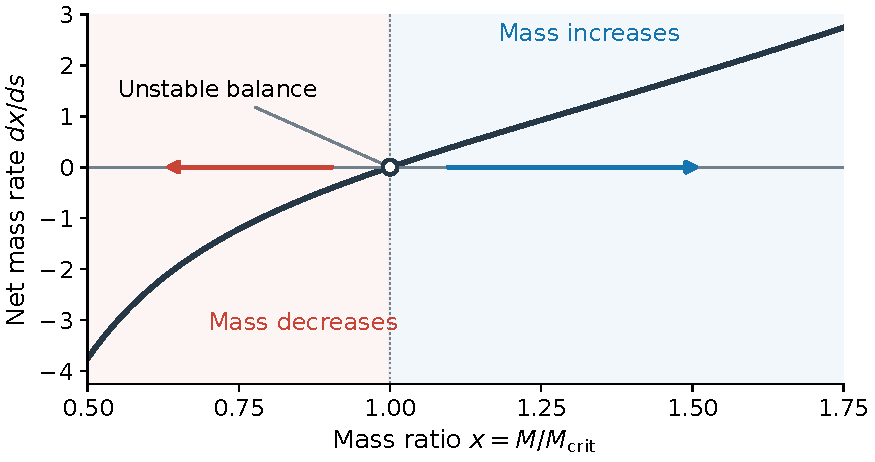
\includegraphics[width=.94\linewidth]{figure1.pdf}
 \caption{\textbf{Equal rates do not restore the mass.} The net dimensionless mass rate crosses zero at $x=1$ with positive slope. Arrows show that masses on either side evolve away from the balance. The curve describes every $A,B>0$ in the fixed-coefficient model.}
 \label{fig:phase}
\end{figure}

\subsection{Exact evolution and terminal times}
Let $x_0=M(0)/\Mcrit$ denote the initial mass ratio. Separating Eq.~\eqref{eq:dimensionless} gives $ds=x^2dx/(x^4-1)$. Partial fractions provide a convenient antiderivative:
\begin{equation*}
 \frac{x^2}{x^4-1}=\frac12\left(\frac1{x^2-1}+\frac1{x^2+1}\right),\qquad
 F(x)=\frac14\ln\left|\frac{x-1}{x+1}\right|+\frac12\arctan x.
\end{equation*}
Integrating from $x_0$ to the current ratio $x$ gives the exact implicit trajectory
\begin{equation}
 \boxed{s=F(x)-F(x_0)}.
 \label{eq:implicit}
\end{equation}
For $0<x_0<1$, this formula applies on $0<x<1$ and the mass decreases. For $x_0>1$, it applies on $x>1$ and the mass increases. The exact equilibrium trajectory is $x(s)=1$. The logarithm in $F$ tends to $-\infty$ as $x\to1$ from either side: a nonconstant trajectory cannot reach or cross $x=1$ in finite time.

For the subcritical branch, $F(0)=0$. We define $t_{\rm evap}$ as the model's formal time to $M=0$. Because $F(x)=[\arctan x-\operatorname{artanh}x]/2$ on $0<x<1$,
\begin{equation}
 \frac{t_{\rm evap}}{\tstar}=-F(x_0)
 =\frac12\bigl[\operatorname{artanh}x_0-\arctan x_0\bigr]
 =\frac{x_0^3}{3}+\frac{x_0^7}{7}+\frac{x_0^{11}}{11}+\cdots.
 \label{eq:evaptime}
\end{equation}
The series is for $0<x_0<1$. Define the pure-evaporation lifetime at the same starting mass as $\taubb(M(0))=M(0)^3/(3B)=\tstar x_0^3/3$. Its associated trajectory is
\begin{equation*}
 M(t)=\bigl[M(0)^3-3Bt\bigr]^{1/3},\qquad 0\leq t\leq\taubb(M(0)).
\end{equation*}
Equation~\eqref{eq:evaptime} shows explicitly how a weak accretion term delays that lifetime:
\begin{equation}
 \frac{t_{\rm evap}}{\taubb(M(0))}
 =1+\frac37x_0^4+O(x_0^8)\quad (x_0\ll1).
 \label{eq:delay}
\end{equation}

For the supercritical branch, $F(x)\to\pi/4$ as $x\to\infty$. We call $t_\infty$ the formal divergence time and $t_{\rm double}$ the time to go from $x_0$ to $2x_0$:
\begin{equation*}
 \frac{t_\infty}{\tstar}=\frac\pi4-F(x_0),\qquad
 \frac{t_{\rm double}}{\tstar}=F(2x_0)-F(x_0),\quad x_0>1.
\end{equation*}
These are mathematical endpoints, not predictions that real matter can sustain unbounded growth or that a semiclassical description remains valid down to zero mass. On either side of equilibrium, terminal times grow as $-\tstar\ln|x_0-1|/4+O(\tstar)$ when $x_0\to1$. Exactly at $x_0=1$ the mass stays fixed, so there is no finite doubling time.

\section{Numerical verification and reference scales}
\subsection{Method and consistency checks}
We numerically integrate Eq.~\eqref{eq:dimensionless} with Python's \texttt{scipy.integrate.solve\_ivp} using DOP853, relative tolerance $10^{-10}$, absolute tolerance $10^{-12}$ and a maximum dimensionless step of $0.02$. To avoid the singular right-hand side near $x=0$, we use $u=x^3$ for decreasing trajectories; to avoid rapidly growing $x$, we use $v=1/x$ for increasing trajectories. These variables obey
\begin{equation*}
 \frac{du}{ds}=3(u^{4/3}-1),\qquad \frac{dv}{ds}=v^4-1,
\end{equation*}
respectively. We stop trajectories at $x=0.05$ or $x=2.2$ using event detection. The filled endpoints in Figure~\ref{fig:trajectories} are numerical cutoffs, not complete evaporation or infinite mass.

For the four plotted curves, the maximum absolute residual $|s-F(x)+F(x_0)|$ at 501 samples per trajectory is $1.67\times10^{-12}$. The largest difference between a numerical cutoff time and the exact time in Eq.~\eqref{eq:implicit} is $4.92\times10^{-13}$. These numbers check the numerical integration of the stated equation; they are not uncertainties on its physical assumptions. The supplied script regenerates the figures and reports the residuals.

\begin{figure}[tbp]
 \centering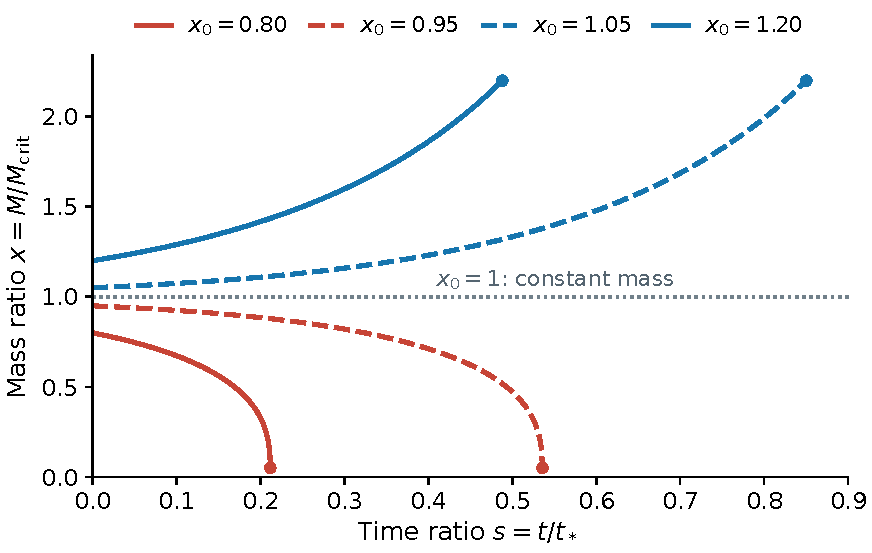
\includegraphics[width=.94\linewidth]{figure2.pdf}
 \caption{\textbf{Perturbations move away from the balance on both sides.} Four numerical trajectories share a dimensionless time axis. Red curves start below $\Mcrit$; blue curves start above it. Dashed curves begin closer to equilibrium and the dotted line is the exact stationary solution. Filled dots mark the plotting cutoffs. For the reference coefficients, one unit of $s$ is $\tstar=2.44\times10^8$ yr, which is distinct from the lifetime at $M_0$.}
 \label{fig:trajectories}
\end{figure}

\subsection{Three distinct timescales}
For the reference coefficients,
\begin{equation*}
 \Mcrit=3.13\times10^{10}\,\mathrm{kg},\qquad
 \tstar=2.44\times10^8\,\mathrm{yr},\qquad
 t_e=6.11\times10^7\,\mathrm{yr}.
\end{equation*}
By contrast, $M_0/\Mcrit=3.20\times10^{-4}$ and $\taubb(M_0)=23.37\,\mathrm h$. The reference hole is far below the near-equilibrium mass represented in Figure~\ref{fig:trajectories}. Its short lifetime cannot be generalized to every subcritical starting mass.

For example, a starting ratio $x_0=0.95$ has a formal evaporation time $0.5360\tstar=1.31\times10^8$ yr. A trajectory starting at $x_0=1.05$ takes $0.8277\tstar=2.02\times10^8$ yr to double. The balance itself stays stationary, so $\tstar$ is not a universal doubling time. At $M_0$, Eq.~\eqref{eq:delay} predicts a fractional lifetime correction of only $4.48\times10^{-15}$; we infer this from the analytic series and do not claim to resolve it with the numerical tolerances used for Figure~\ref{fig:trajectories}.

\section{Physical interpretation and limitations}
\subsection{Changing the medium shifts an unstable balance}
The balance depends on the medium as
\begin{equation*}
 \Mcrit=\left(\frac{Bc_\infty^3}{4\pi\lambda\rho_\infty G^2}\right)^{1/4}.
\end{equation*}
At fixed $B$ and $\lambda$, changing $\rho_\infty$ by a factor $R$ changes $\Mcrit$ by $R^{-1/4}$; changing $c_\infty$ by a factor $S$ changes it by $S^{3/4}$. Neither change makes $f'(\Mcrit)$ negative.

Let $A_{\rm ref}$ denote the coefficient of our illustrative medium, and let $Q=A/A_{\rm ref}$ while $B$ stays fixed. Equality between the balance mass and $M_0$ would require
\begin{equation*}
 Q_{\rm bal}=\frac{B}{A_{\rm ref}M_0^4}=9.56\times10^{13}.
\end{equation*}
If density alone changed while sound speed and $\lambda$ were artificially held fixed, this would correspond to $\rho_{\rm req}=9.56\times10^{16}\,\mathrm{kg\,m^{-3}}$. The extrapolation is not a proposed material: at such a change the equation of state and accretion model must be reconsidered. Figure~\ref{fig:medium} plots coefficient sensitivity, not a map of realizable substances.

\begin{figure}[tbp]
 \centering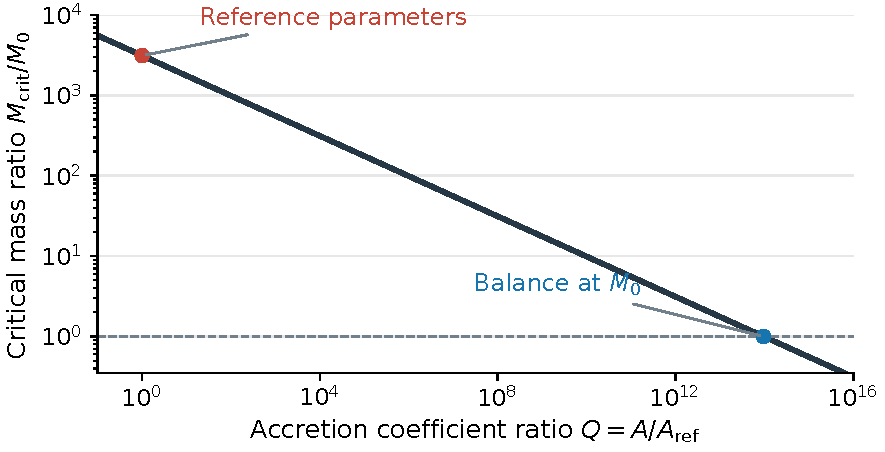
\includegraphics[width=.94\linewidth]{figure3.pdf}
 \caption{\textbf{Increasing accretion strength moves, but never stabilizes, the balance.} At fixed $B$, $\Mcrit/M_0=3126.65\,Q^{-1/4}$. The reference point is $Q=1$ and equality $\Mcrit=M_0$ occurs at $Q=9.56\times10^{13}$. Every point on the curve has the positive derivative in Eq.~\eqref{eq:derivative}.}
 \label{fig:medium}
\end{figure}

\subsection{The Eddington force balance is a different condition}
For an outward luminosity $L$, suppose the material has an effective flux-mean opacity $\kappa_F$. The idealized outward radiative acceleration is $a_{\rm rad}=\kappa_F L/(4\pi r^2c)$. Equating it to the inward gravitational acceleration $GM/r^2$ defines
\begin{equation*}
 L_E=\frac{4\pi GMc}{\kappa_F}.
\end{equation*}
If we insert $L=K/M^2$ from Eq.~\eqref{eq:power}, the formal force-balance mass $M_E$ obeys
\begin{equation*}
 M_E=\left(\frac{\kappa_FK}{4\pi Gc}\right)^{1/3},\qquad
 \frac{a_{\rm rad}}{a_{\rm grav}}=\left(\frac{M_E}{M}\right)^3.
\end{equation*}
This cube-root balance depends on opacity; the fourth-root mass balance in Eq.~\eqref{eq:mcrit} depends on the accretion coefficient. They are not generally equal. As a formal example, the low-energy Thomson opacity of ionized hydrogen $\kappa_F=\sigma_T/m_p$ yields $M_E=3.83\times10^{10}\,\mathrm{kg}$ and a force ratio of $5.63\times10^{10}$ at $M_0$. Using this opacity unchanged for a TeV-scale, multispecies Hawking spectrum is unjustified. The coupling fraction and the medium's frequency-dependent absorption and scattering require a separate calculation~\cite{ciotti}.

\subsection{What carries over to other models?}
The unstable equilibrium survives any \emph{constant} positive rescaling of $A$ or $B$. For example, replacing $B$ by $\eta B$ with fixed $\eta>0$ changes $\Mcrit$ by $\eta^{1/4}$ and $t_e$ by $\eta^{-1/4}$ at fixed $A$; at a fixed initial mass the pure-evaporation lifetime scales as $\eta^{-1}$.

A general local test shows where this conclusion stops. Write $\dot M=C(M)-E(M)$ with positive gain and loss rates. Suppose they balance at $M_*$ with $C(M_*)=E(M_*)=R_*>0$. Define logarithmic slopes $p=d\ln C/d\ln M$ and $q=d\ln E/d\ln M$ at $M_*$. Then
\begin{equation*}
 \left.\frac{d\dot M}{dM}\right|_{M_*}=\frac{R_*}{M_*}(p-q).
\end{equation*}
Here $p=2$ and $q=-2$. Other laws can give a different sign: $p<q$ gives local asymptotic stability, while $p=q$ needs higher-order analysis. If gas temperature, density or black hole spin also evolve, one must test the stability of the full coupled system.

The main physical uncertainties are the continuum Bondi approximation at the reference scale, radiation-dependent heating and flow, realistic Hawking spectra, finite reservoirs and additional degrees of freedom such as angular momentum or charge. None is contained in Eq.~\eqref{eq:mass}. The quantity $M_0c^2$ is likewise not guaranteed useful energy, because collection efficiency and weakly interacting emissions are outside this calculation.

\section{Conclusion}
Within the fixed-coefficient law $\dot M=AM^2-B/M^2$ for positive $A$ and $B$, there is one positive balance and it is unstable. The exact solution and independently integrated trajectories show motion away from it on both sides. The model also distinguishes a short blackbody lifetime far below equilibrium from a slow departure when the initial mass lies very close to equilibrium.

The supported conclusion is specific: passive mass balance is unstable in this idealized Hawking--Bondi equation. A natural physical extension is to calculate how radiation changes the surrounding medium and accretion rate, then test the resulting coupled dynamics. Rotation would require simultaneous evolution of mass and angular momentum rather than a replacement of the temperature alone.

\appendix
\section{The coefficient in the Hawking temperature}\label{app:temperature}
We use regular Euclidean Schwarzschild geometry to recover the coefficient in Eq.~\eqref{eq:temperature}~\cite{gibbons,genolini}. The Lorentzian line element, in a conventional exterior coordinate chart, is
\begin{equation*}
 d\ell^2=-f(r)c^2dt^2+\frac{dr^2}{f(r)}+r^2d\Omega^2,
 \quad f(r)=1-\frac{r_s}{r},\quad r_s=\frac{2GM}{c^2}.
\end{equation*}
After continuing $t=-it_E$, set $r=r_s+\epsilon$ near the horizon and define $R=2\sqrt{r_s\epsilon}$. To leading order in $\epsilon/r_s$,
\begin{equation*}
 f\simeq\frac{\epsilon}{r_s}=\frac{R^2}{4r_s^2},\qquad
 \frac{dr^2}{f}\simeq dR^2,\qquad
 d\ell_E^2\simeq dR^2+R^2d\theta^2,
 \quad\theta=\frac{ct_E}{2r_s}.
\end{equation*}
For this plane to be smooth at $R=0$, $\theta$ must have period $2\pi$. Hence $t_E$ has period $\Delta t_E=4\pi r_s/c=8\pi GM/c^3$. Imaginary-time evolution $e^{-H\Delta t_E/\hbar}$ has the thermal period $\Delta t_E=\hbar/(k_BT_H)$, yielding
\begin{equation*}
 T_H=\frac{\hbar}{k_B\Delta t_E}=\frac{\hbar c^3}{8\pi GMk_B}.
\end{equation*}
This argument fixes the temperature of the regular thermal Schwarzschild state. On its own it does not calculate outgoing flux after collapse or transmission through the exterior potential; those need a quantum-field and greybody calculation~\cite{hawking,page}.

\section{Reference values and reproducibility}\label{app:values}
We use SI units with $G=6.67430\times10^{-11}\,\mathrm{m^3kg^{-1}s^{-2}}$, $c=299792458\,\mathrm{m\,s^{-1}}$, $h=6.62607015\times10^{-34}\,\mathrm{J\,s}$, $k_B=1.380649\times10^{-23}\,\mathrm{J\,K^{-1}}$, $\hbar=h/(2\pi)$, and one year of 365.25 days. The medium parameters are defined in Sec.~2.2. Displayed quantities are rounded; calculations use full floating-point precision.

\begin{table}[htbp]
\centering\small
\caption{Reference values in the stated blackbody and fixed-medium model. The evaporation rate is a positive magnitude.}\label{tab:values}
\begin{tabular}{@{}p{.58\linewidth}r l@{}}
\toprule
Quantity & Value & Unit\\
\midrule
Initial mass $M_0$ & $1.00\times10^7$ & kg\\
Horizon radius $r_s(M_0)$ & $1.49\times10^{-20}$ & m\\
Temperature $T_H(M_0)$ & $1.23\times10^{16}$ & K\\
Blackbody luminosity $\Pbb(M_0)$ & $3.56\times10^{18}$ & W\\
Pure-evaporation lifetime $\taubb(M_0)$ & $23.37$ & h\\
Bondi scale $r_B(M_0)$ & $2.97\times10^{-10}$ & m\\
Accretion coefficient $A$ & $4.15\times10^{-27}$ & $\mathrm{kg^{-1}s^{-1}}$\\
Evaporation coefficient $B$ & $3.96\times10^{15}$ & $\mathrm{kg^3s^{-1}}$\\
Accretion rate $AM_0^2$ & $4.15\times10^{-13}$ & $\mathrm{kg\,s^{-1}}$\\
Evaporation rate $B/M_0^2$ & $39.6$ & $\mathrm{kg\,s^{-1}}$\\
Critical mass $\Mcrit$ & $3.13\times10^{10}$ & kg\\
Time scale $\tstar$ & $2.44\times10^8$ & yr\\
Perturbation e-folding time $t_e$ & $6.11\times10^7$ & yr\\
\bottomrule
\end{tabular}
\end{table}

The accompanying repository contains \texttt{main.tex}, \texttt{reproduce.py}, three vector figures in \texttt{figures/} and \texttt{results.json}. Running \texttt{python3 reproduce.py} regenerates the figures, constants and integration checks. Running \texttt{pdflatex main.tex} twice rebuilds this paper.

\begin{thebibliography}{9}
\bibitem{hawking} S. W. Hawking, ``Particle creation by black holes,'' \emph{Communications in Mathematical Physics} \textbf{43}, 199--220 (1975). \href{https://doi.org/10.1007/BF02345020}{doi:10.1007/BF02345020}.
\bibitem{gibbons} G. W. Gibbons and S. W. Hawking, ``Action integrals and partition functions in quantum gravity,'' \emph{Physical Review D} \textbf{15}, 2752--2756 (1977). \href{https://doi.org/10.1103/PhysRevD.15.2752}{doi:10.1103/PhysRevD.15.2752}.
\bibitem{genolini} P. Benetti Genolini, ``Introduction to black hole thermodynamics,'' lecture notes (2025). \href{https://arxiv.org/abs/2512.24929}{arXiv:2512.24929}.
\bibitem{page} D. N. Page, ``Particle emission rates from a black hole: Massless particles from an uncharged, nonrotating hole,'' \emph{Physical Review D} \textbf{13}, 198--206 (1976). \href{https://doi.org/10.1103/PhysRevD.13.198}{doi:10.1103/PhysRevD.13.198}.
\bibitem{macgibbon} J. H. MacGibbon and B. R. Webber, ``Quark- and gluon-jet emission from primordial black holes: The instantaneous spectra,'' \emph{Physical Review D} \textbf{41}, 3052--3079 (1990). \href{https://doi.org/10.1103/PhysRevD.41.3052}{doi:10.1103/PhysRevD.41.3052}.
\bibitem{bondi} H. Bondi, ``On spherically symmetrical accretion,'' \emph{Monthly Notices of the Royal Astronomical Society} \textbf{112}, 195--204 (1952). \href{https://doi.org/10.1093/mnras/112.2.195}{doi:10.1093/mnras/112.2.195}.
\bibitem{ciotti} L. Ciotti and J. P. Ostriker, ``Free-free absorption effects on Eddington luminosity'' (2003). \href{https://arxiv.org/abs/astro-ph/0312490}{arXiv:astro-ph/0312490}.
\end{thebibliography}

\end{document}
